\section*{Perulangan}

\par
Didalam python, kita dapat melakukan proses perulangan. contohnya sebagai berikut.


\begin{enumerate}
	\item buka spyder lalu tulis script sebagai berikut.
	\begin{figure} [h]
	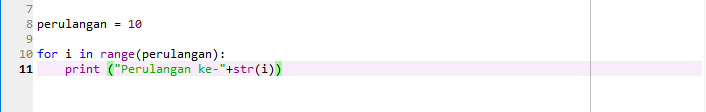
\includegraphics[width=9cm]{loop/loop1.png}
	\centering
	\end{figure}

\item kalian dapat mengisi jumlah loop yang akan dilakukan sesuai dengan keinginan kalian
	
    \item maka hasil ke layar akan menjadi sebagai berikut
	\begin{figure} [h]
	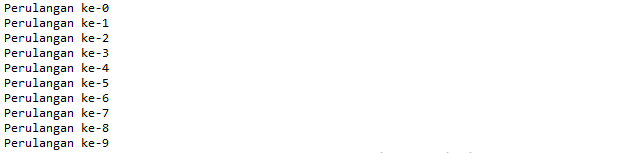
\includegraphics[width=9cm]{loop/loop2.png}
	\centering
	\end{figure}
	
	

\end{enumerate}